\section{Discussion}
\label{chap:Discussion}

\subsection{Part A}
\label{chap:PartA}

\subsubsection{Ordinary Least Squares, Ridge regression and Stochastic Gradient Descent on terrain's heights GeoTIF image-data}
\label{chap:Ordinary Least Squares, Ridge regression and Stochastic Gradient Descent on terrain's heights GeoTIF image-data}

\qquad \, We start part A of this project with a re-capitulation of \href{https://github.com/fabiorodp/UiO-FYS-STK4155/blob/master/Project1}{Project 1}, part F and G, where a GeoTIF terrain image, containing the heights of a region near Stavanger/Norway, was extracted and examined on Ordinary Least Squares (OLS) and Ridge regression models. On that occasion, we generated two sets of explanatory variables ($\boldsymbol{x1}$, $\boldsymbol{x2}$), with values between 0 and 1, and utilized them on the design matrix ($\boldsymbol{X}$) function that performed a polynomial transformation with a degree equals 10 for OLS and 11 for Ridge. The response variable set ($\boldsymbol{z}$) had space (number of samples or size of the sliced image) of 15 (15x15 pixels). Lastly, the testing MSE (mean squared error) scores obtained were 1.11 and 1.44 for OLS and Ridge, respectively.\\

Now, we perform a Stochastic Gradient Descent (SGD) utilizing the same generated data as above. It is essential to say that we do not scale the data-sets because of possible crashes during the gradient computations. The \href{https://github.com/fabiorodp/UiO-FYS-STK4155/blob/master/Project2/package/gradient_descent.py}{gradient\_descent.py} under the \href{https://github.com/fabiorodp/UiO-FYS-STK4155/tree/master/Project2/package}{Project2/package/} directory has the algorithms for GDM and Mini-SGDM.\\

Our first experiment for SGD is a combination of parameters incorporated at the \href{https://github.com/fabiorodp/UiO-FYS-STK4155/tree/master/Project2/package}{Project2/package/} directory, file name \href{https://github.com/fabiorodp/UiO-FYS-STK4155/blob/master/Project2/package/studies.py}{studies.py} and class name \textit{SearchParametersMiniSGDM}. We run the \textit{SearchParametersMiniSGDM} class to find the best constant learning rate $\eta$ = [0.02, 0.01, 0.005, 0.001, 0.0005] as a function of the number of interactions epochs=[100, 500, 1000, 5000, 10000]. The model applied is the MiniSGDM, which is an SGD when the number of batches is equal to 1, gamma=0, lambda=0, and decay=0.\\

The results are as follows:

\begin{figure}[H]
\label{fig:figA1}
\centering
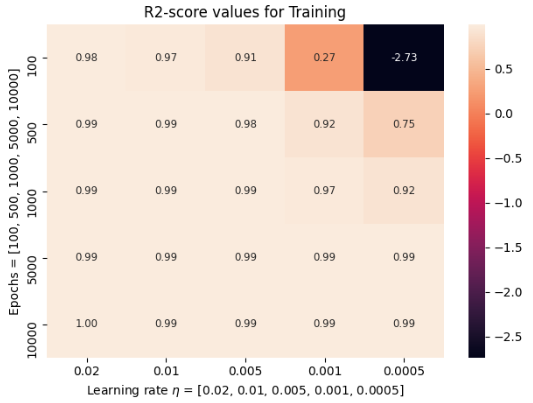
\includegraphics[width=7cm]{heatmapA1}
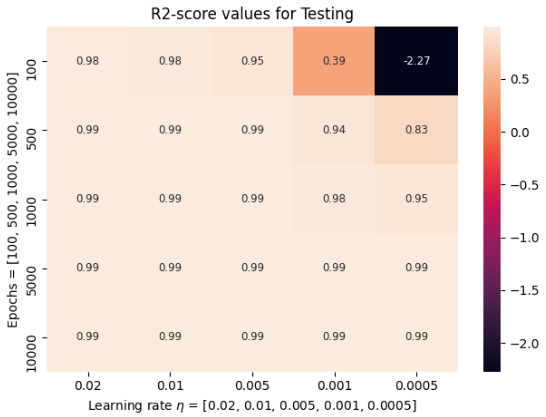
\includegraphics[width=7cm]{heatmapA2}
\caption{Heat-map containing the R2-score training and testing results of a Grid-Search with Learning rates = [0.02, 0.01, 0.005, 0.0001, 0.0005] and epochs = [100, 500, 1000, 5000, 10000].}
\end{figure}

As one can see, the design matrix ($\boldsymbol{X}$) with degree equals to 10 explains the response variable ($\boldsymbol{z}$) at a rate of 99 percent, according to the r2-scores. In other words, these results suggest that the input polynomials translate almost entirely the output heights of the terrain region studied.

\begin{figure}[H]
\label{fig:figA2}
\centering
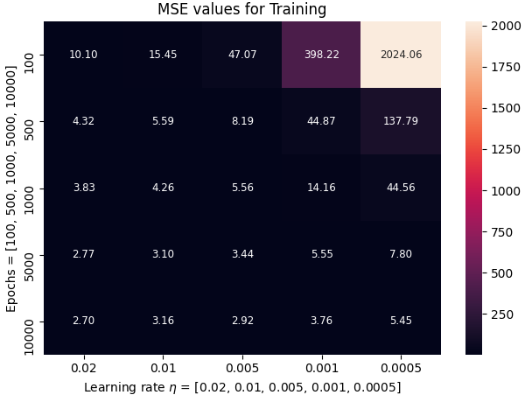
\includegraphics[width=7cm]{heatmapA3}
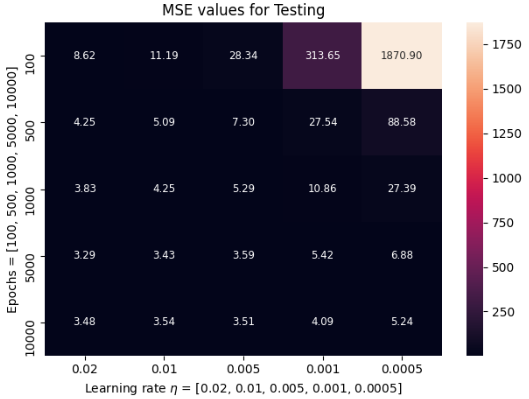
\includegraphics[width=7cm]{heatmapA4}
\caption{Heat-map containing the MSE training and testing results of a Grid-Search with Learning rates = [0.02, 0.01, 0.005, 0.0001, 0.0005] and epochs = [100, 500, 1000, 5000, 10000]. }
\end{figure}

The results from training and testing MSE heat-maps indicate as the best scores are 2.77 and 2.99 for learning rates 0.02 and epochs 10.000. Notice that as the number of epochs increases, the MSE scores decreases indicating that the gradient of the loss-function is in the direction of the minimum local/global as expected. 

\begin{figure}[H]
\label{fig:figA3}
\centering
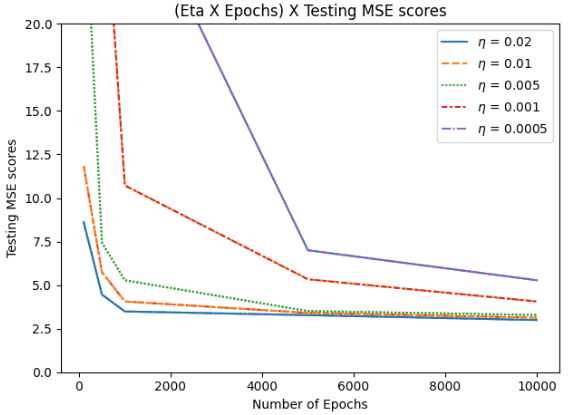
\includegraphics[height=5cm]{linesA1}
\caption{Line-plot showing (Eta x Epochs) X Testing MSE scores. }
\end{figure}

\hyperref[fig:figA3]{Line-plots above} evince that the accuracy for the learning rates converges to its best score near 1.000 epochs. Therefore, we choose the number of epochs equals 1.000 as the parameter's benchmarks on futures experiments.

\subsubsection{Tuning computation's cost (mini-batches)}
\label{chap:Tuning computation's cost (mini-batches)}

\qquad \, The SGD method with a unique mini-batch is costly for computations while fitting the model. The algorithm stochastically chooses a single vector of features from the sample space, calculates the gradient, and updates the weights. This process is repeated for as many samples in the design matrix ($\boldsymbol{X}$) for every epoch. It turns out that the number of computations sky rocks and the entire fitting takes a long time to complete, as shown on the heat-map below:

\begin{figure}[H]
\label{fig:figA4}
\centering
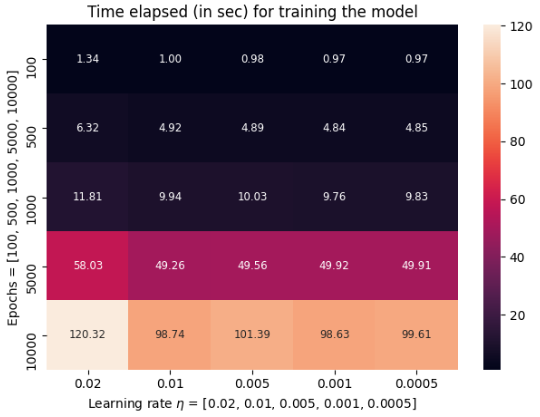
\includegraphics[width=8cm]{heatmapA5}
\caption{Heat-map containing the fitting time (in seconds) of the previous Grid-Search on \hyperref[fig:figA1]{Fig.1} and \hyperref[fig:figA2]{Fig.2}.}
\end{figure}

It is evident that as the number of epochs is high, the computations' costs are higher. For example, our model's fitting time takes approx. 1 seconds to run when the epoch number is 100. On the other hand, when the epoch is 10.000, the fitting time takes approx. 100 seconds.\\

To avoid the cost of this expensive computation, we introduce the mini-batches technique. Instead of stochastically choosing only one vector of features from the training sample, the algorithm chooses feature vectors blocks.\\

Therefore, we perform a \textit{SearchParametersMiniSGDM} for the parameters etas=[0.01, 0.005, 0.001, 0.0005] and batch\_sizes=[1, 5, 10, 15, 20], using our bench-marked epoch value equals to 1.000, and analyse the testing MSE performance and fitting's time on the heat-maps below:

\begin{figure}[H]
\label{fig:figA5}
\centering
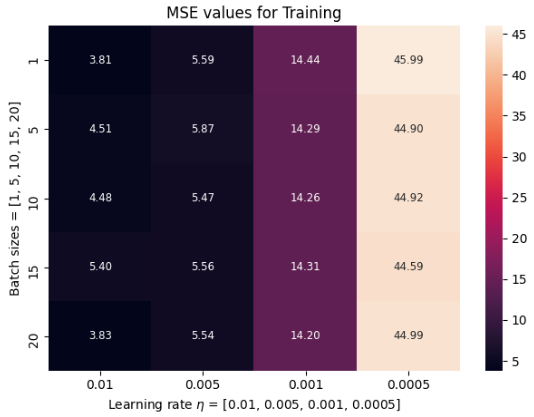
\includegraphics[width=7cm]{heatmapA6}
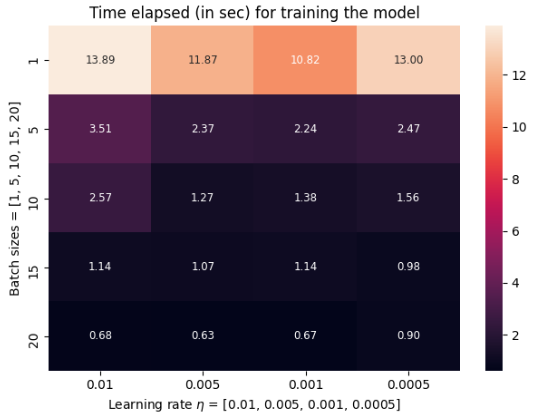
\includegraphics[width=7cm]{heatmapA7}
\caption{Left heat-map shows the testing MSE scores for each search. Right heat-map shows the fitting's time for each search.}
\end{figure}

For a single vector of features (batch\_size=1), the elapsed fitting's times are above 10 seconds. Under blocks of feature vectors (mini-batches), the elapsed fitting times have a tremendous reduction without losing much the accuracy. For example, the case with learning rate=0.01 and batch-size=1 got MSE equals 3.81, and fitting's time equals 13.89 seconds, however for the same learning rate=0.01, but batch\_size=20, the fitting's time was approx. 20 times faster and with almost the same accuracy of 3.83.

\begin{figure}[H]
\label{fig:figA6}
\centering
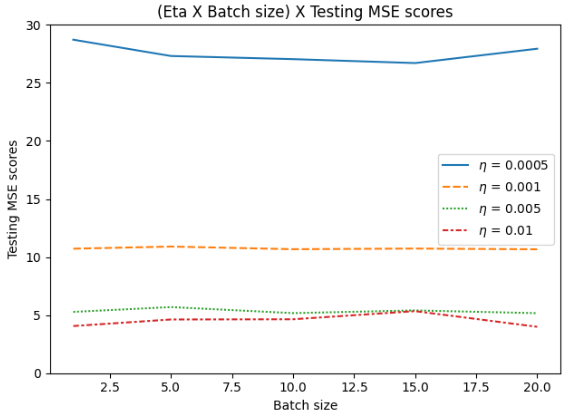
\includegraphics[height=5cm]{linesA2}
\caption{Line.plot containing (Eta x Batch size) X testing MSE.}
\end{figure}

\hyperref[fig:figA6]{Fig.11} shows that the constant learning rate $\eta$=0.01 performs better than the other learning rates. It has constant accuracy for all batch sizes tested. Besides, we see that batch\size=10 is the sweet spot for $\eta$=0.01 because it is where the accuracy starts to worsen.\\

Hence, we define our bench-marked parameters epochs=1.000 and batch\_size=10 for futures examinations.

\subsubsection{Learning rate decay and tuning decay}
\label{chap:Learning rate decay and tuning decay}

\qquad \, There are many ways to optimize the learning rate to find more accurate predictions. As studied in \hyperref[chap:Gradient Decedent]{Gradient Descent theory}, the learning rate ($\eta$) is a hyper-parameter that manages the model's change in response to the MSE each time the model's coefficients (weights) are updated.\\

Now, we apply a technique that reduces the learning rate value according to the number of epochs, studied in \hyperref[chap:Learning Rate with decay]{Learning rate decay}. To do that, we introduce a constant parameter called decay.\\

Thus, we run a \textit{SearchParametersMiniSGDM} with the parameters etas=[0.35, 0.3, 0.25, 0.2, 0.01] and decays=[10**-1, 10**-2, 10**-3, 10**-4, 10**-5], using our bench-marked epoch=1.000 and batch-size=10, to find the best testing MSE score for an eta as a function of a decay value:

\begin{figure}[H]
\label{fig:figA7}
\centering
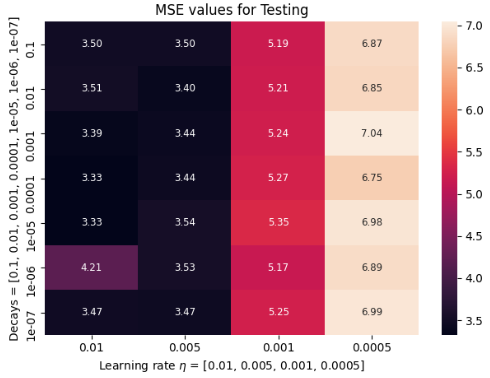
\includegraphics[height=5cm]{heatmapA8}
\caption{Heat-map showing the testing MSE scores for learning rates as function of decays.}
\end{figure}

With this decay technique, we were able to increase the learning rate without breaking the gradient calculation. Therefore, the best testing MSE achieved was 4.32 for learning rate=0.3 and decay=0.001.\\

Hence, we include decay=0.001 and eta0=0.3 to our bench-marked parameters epochs=1.000, batch\_size=10. We will try to beat the testing MSE of 4.32 obtained in this section by introducing mini-batch SGD momentum (gamma) and 'l2' regularization in the following sub-sections.

\subsubsection{SGD with momentum and tuning gamma}
\label{chap:SGD with momentum and tuning gamma}

\qquad \, This subsection will try to overcome the testing MSE of 4.32 by applying another type of Mini-batch Stochastic Gradient Descent, so-called Mini-batch SGD with momentum. A new parameter gamma is introduced, as explained in the theory section in \hyperref[chap:BGD, SGD and Mini-batch SGD with momentum]{"BGD, SGD and Mini-batch SGD with momentum"}. We use different values of gamma=[0, 0.1, 0.2, 0.25, 0.3, 0.35, 0.4, 0.5, 0.6] and run the model \href{https://github.com/fabiorodp/UiO-FYS-STK4155/blob/master/Project2/package/gradient_descent.py}{MiniSGDM} with the bench-marked parameters obtained from the previous subsections, decay=0.001, eta0=0.3, epochs=1.000 and batch\_size=10.

\begin{figure}[H]
\label{fig:figA8}
\centering
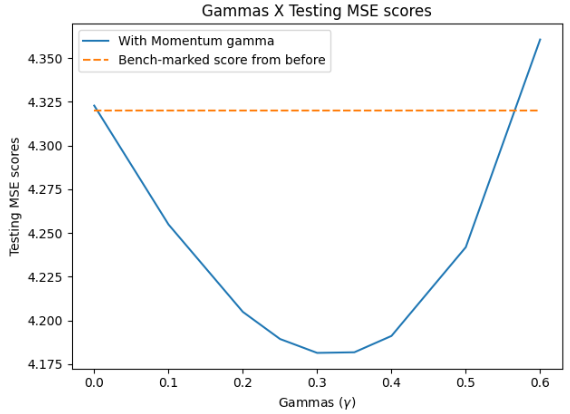
\includegraphics[width=7cm]{linesA3}
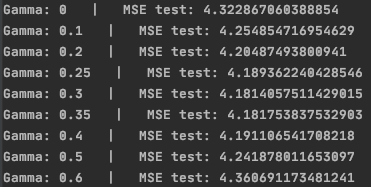
\includegraphics[width=7cm]{outputA1}
\caption{Left line-plot containing the MSE values as function of gammas. Right output of accuracy values for gammas.}
\end{figure}

As shown, the Mini-batch Stochastic Gradient Descent with momentum overcome our bench-marked score of 4.32, reaching 4.18 when gamma parameter is 0.3.\\

Hence, we include gamma=0.3 to our bench-marked parameters decay=0.001, eta0=0.3, epochs=1.000, batch\_size=10. We will try to beat the testing MSE of 4.1814 obtained in this section by introducing 'l2' regularization (Ridge lambda) in the next sub-section.

\subsubsection{'L2' regularization and tuning lambda}
\label{chap:'L2' regularization and tuning lambda}

\qquad \, This subsection will try to overcome the testing MSE of 3.65 by applying the l2 regularization (Ridge). A new parameter lambda is introduced, as explained in the theory section of \href{https://github.com/fabiorodp/UiO-FYS-STK4155/blob/master/Project1}{Project 1}. We use different values of lambda=[0, 10**-9, 10**-6, 10**-4] and run the model \href{https://github.com/fabiorodp/UiO-FYS-STK4155/blob/master/Project2/package/gradient_descent.py}{MiniSGDM} with the bench-marked parameters obtained from the previous subsections, gamma=0.3, decay=0.001, eta0=0.3, epochs=1.000 and batch\_size=10.

\begin{figure}[H]
\label{fig:figA9}
\centering
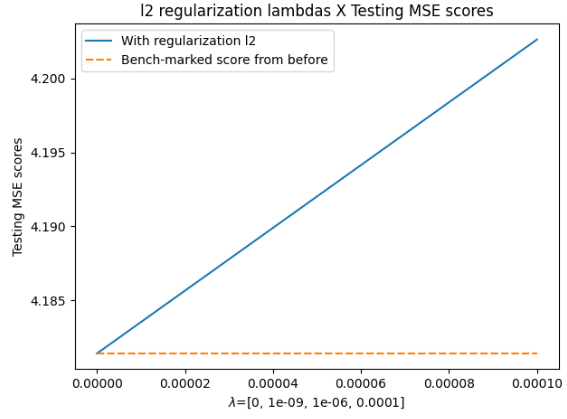
\includegraphics[width=8cm]{linesA4}
\caption{Line-plot containing the MSE values as function of lambdas.}
\end{figure}

As exhibited, the 'l2' regularization did not make any improvement overcoming our bench-marked testing accuracy of 4.1814.

\subsection{Part B and C}
\label{chap:Part B and C}

\qquad \, In part B and C of this report, we will discuss the application of our own Feed Forward Deep Neural Network (DNN) with the back-propagation method on a regression problem. The data-set applied on DNN will be the GeoTIF terrain image utilized in part A. It is essential to mention that the descriptive data-set will not be submitted to a design matrix function, as we did in part A, because the DNN should identify possible linearity by itself. Also, the targets will not be scaled, as we did not do that on "Project 1" and part A. These choices are because of comparisons propose as the performances between OLS, Ridge, Mini-batch SGDM and DNN will be distinguished, and we want to feed the models with almost the same complexities as fed before.\\

The cost-function employed is the Mean Squared Error (MSE) due to the regression nature of this kind of problem. Also, as explained on the \hyperref[chap:Deep Neural Networks]{DNN theory topic}, the MSE function matches very well on models that use gradient descent because of MSE's convexity and continuity aspects.\\

Moreover, the activation function for the hidden layers will be \hyperref[chap:Sigmoid]{Sigmoid} on the first experiments and then \hyperref[chap:Hyperbolic tanh]{Tanh} and \hyperref[chap:Rectified Linear Unit]{Relu}. The output layer's activation function will be "identity" because DNN for regression cases does not use an activation function for output values.\\

The way that the models' weights and biases are initialized is through Gaussian distribution, but another method so-called \hyperref[chap:Xavier and He weights initialization method]{"Xavier method"} will be explored. Both approaches are explained in detail in the theory section.\\

Finally, the number of epochs tested in this section will be fixed at 500 because of computation costs. The batch\_size will also be fixed at the samples' length in training data due to the best metrics than mini-batches.

\subsubsection{Number of Neurons Vs Learning rates for 1 hidden layer Sigmoid}
\label{chap:Number of Neurons Vs Learning rates for 1 hidden layer Sigmoid}

\qquad \, At the beginning of part B of this report, we will employ a one-layer neural network to analyze different vital topics regarding the number of neurons, learning rate, epoch, cost error, decay, and 'l2' regularization.\\

The Python function called one\_hidden\_layer\_sigmoid at file \href{https://github.com/fabiorodp/UiO-FYS-STK4155/blob/master/Project2/partBandC.py}{partBandC.py} in the directory \href{https://github.com/fabiorodp/UiO-FYS-STK4155/blob/master/Project2/}{Project2/} will perform the following experiments and return the results we will discuss here.\\

First, we would like to find the best number of neurons as a function of a learning rate ($\eta$) value. For that, n\_neurons = [10, 20, 30, 40, 50, 75, 100, 125, 150] and etas = [0.99, 0.9, 0.8, 0.7, 0.6, 0.5] are defined and performed on our class \textit{SearchParametersDNN} in \href{https://github.com/fabiorodp/UiO-FYS-STK4155/blob/master/Project2/package/studies.py}{studies.py} at directory \href{https://github.com/fabiorodp/UiO-FYS-STK4155/blob/master/Project2/package/}{package/}. This class method fits our Multi-layer perceptron (MLP) function with a combination of the previous parameters, one by one, to identify which one returns the best metrics as follows:

\begin{figure}[H]
\label{fig:B1}
\centering
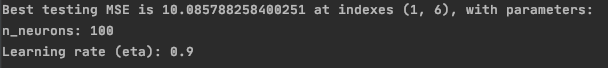
\includegraphics[width=12cm]{B1}
\caption{Output for printing best combination of metrics.}
\end{figure}

This first output shows that the best combination of parameters is neurons = 100 and learning rate = 0.9, which obtained testing MSE at 10.0857.

\begin{figure}[H]
\label{fig:B2}
\centering
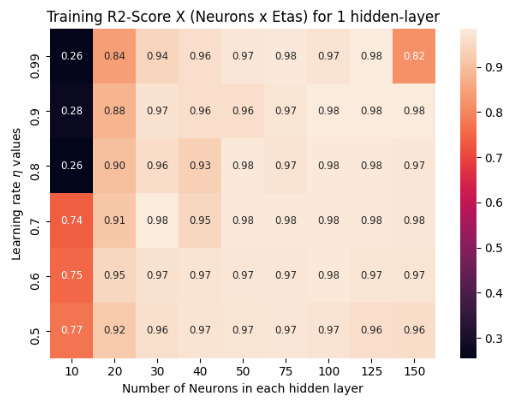
\includegraphics[height=5cm]{B2}
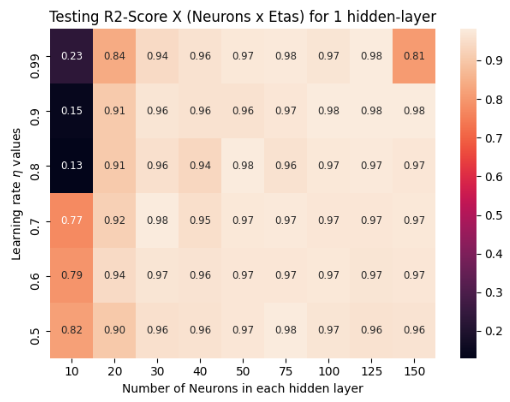
\includegraphics[height=5cm]{B3}
\caption{Heat-maps containing the R2-score training and testing results.}
\end{figure}

\begin{figure}[H]
\label{fig:B3}
\centering
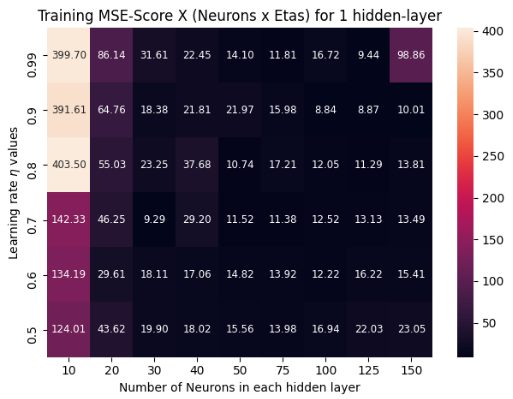
\includegraphics[height=5cm]{B4}
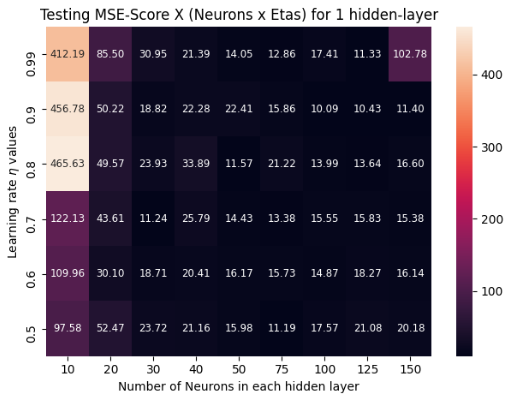
\includegraphics[height=5cm]{B5}
\caption{Heat-maps containing the MSE-score training and testing results.}
\end{figure}

The results are promising because the model reached r2-score around 99 percent for only one hidden-layer. The best training and testing MSE accuracies were 8.84 and 10.09, respectively, at neurons = 100 and $\eta$ = 0.9. Observe that when the neurons and learning rates are smaller or larger than 100 and 0.9, the model gets worse scores, indicating that the parameters are optimized.

\begin{figure}[H]
\label{fig:B4}
\centering
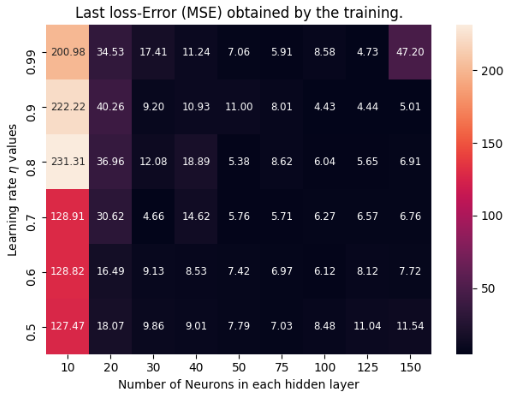
\includegraphics[height=5.5cm]{B6}
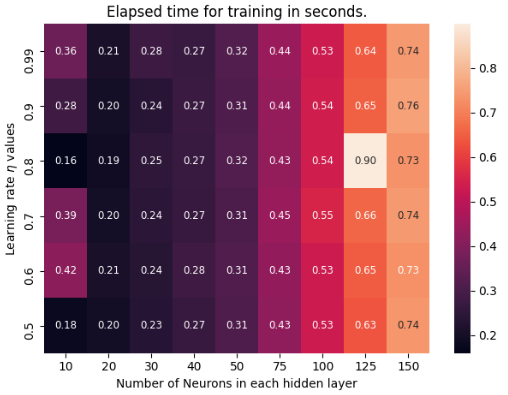
\includegraphics[height=5.5cm]{B7}
\caption{Heat-maps containing the loss-error for the last training epoch (left) and elapsed training times (right).}
\end{figure}

The loss-error is the MSE score measured for every Feed-Forward process for every epoch during training. As shown above, the best loss-error for the last training epoch at neurons = 100 and $\eta$=0.9 likewise was the smallest/best with a 4.43 score. This score is overestimated because the training and testing MSE scores were higher in \hyperref[fig:B3]{Figure 17}. Besides, as the number of neurons is high, the time elapsed for training is more considerable.

\begin{figure}[H]
\label{fig:B5}
\centering
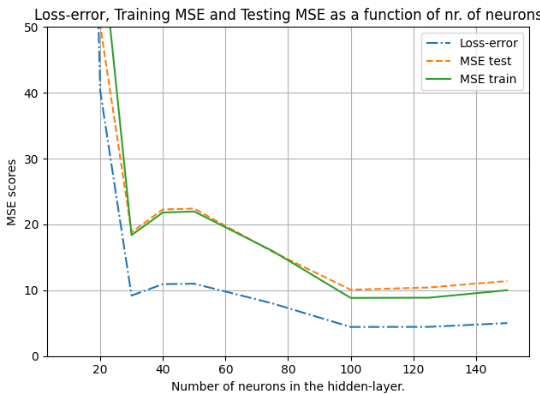
\includegraphics[height=5.5cm]{B8}
\caption{Line-plot containing the loss-error, training and testing MSE scores for $\eta$=0.9 and different neurons values.}
\end{figure}

\hyperref[fig:B5]{The previous figure} shows that our parameter's sweet spot is 100 for the number of neurons. This parameter is optimal because it reached the best score in the searching and where the bias and variance of the model are the lowest since loss-error, training and testing lines are in the smallest score and closest among each other. Besides, an increase in the variance happens when the complexity number of neurons increases above 100, where the scores worsen, and the difference among loss-error, training and testing increases.

\subsubsection{Accuracy analysis and epochs analysis}
\label{chap:Accuracy analysis and epochs analysis}

\qquad \, Considering our best model from the previous sub-topic, we can analyze each epoch's accuracy score's evolution by the succeeding line-plots:

\begin{figure}[H]
\label{fig:B6}
\centering
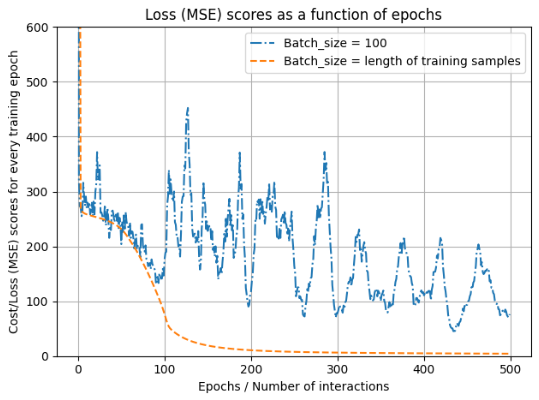
\includegraphics[height=5.5cm]{B9}
\caption{Line-plot containing the cost/loss-error for every training epoch.}
\end{figure}

At the beginning of the fitting, the accuracy is terrible because of the randomness initiation of the layers' weights and biases. As long as the epochs are processed, our gradient descent does an excellent task, converging and decreasing to the local or global minimum score.\\

It is imperative to say that we were using the parameter batch\_size equals the number of samples of the training data. This parameter makes the cost curve above being smooth due to the batch gradient descent essence, as explained in \hyperref[chap:Mini-batch Stochastic Gradient Decedent]{theory}.\\

chap:Mini-batch Stochastic Gradient Decedent

However, when we define batch\_size equals 100, less than the number of samples of the training data, then the cost curve will differ, being choppy due to the Stochastically nature of the mini-batches choices. Nonetheless, the gradient descent still performs very well, converging the cost to its minimum as expected. This option of batch\_size gains a lot in speedy of the computation, likewise explained in \hyperref[chap:Mini-batch Stochastic Gradient Decedent]{theory section"}, and it is ideal for extensive explanatory data with a considerable number of samples and features.

\subsubsection{Tuning the learning rate, decay and "l2" regularization}
\label{chap:Tuning the learning rate, decay and "l2" regularization}

\qquad \, We will tune the parameters learning rate ($\eta$), decay and 'l2' Ridge regularization lambda. Remember that the explanations about each parameter are in the theory section. For this optimization, we choose different values for etas = [0.99, 0.95, 0.9, 0.85, 0.8, 0.7, 0.6, 0.5], decays = [0, 10 ** -9, 10 ** -8, 10 ** -7, 10 ** -6, 10 ** -5, 10 ** -4, 10 ** -3, 10 ** -2, 10 ** -1] and lambdas = [0, 10 ** -9, 10 ** -8, 10 ** -7, 10 ** -6, 10 ** -5, 10 ** -4, 10 ** -3, 10 ** -2, 10 ** -1], and then perform the MLP model for each combination of parameters. The printed output shows the best parameters and testing MSE score for the best combination:

\begin{figure}[H]
\label{fig:B7}
\centering
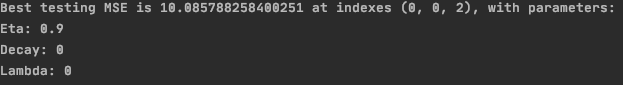
\includegraphics[width=12cm]{B10}
\caption{Printed output containing the best parameters of the searching.}
\end{figure}

This output confirms that the learning rate equal to 0.9 acquired before is optimized. Besides, the decay and lambda parameters did not help the MLP model overcome the testing MSE score of 10.085.

\begin{figure}[H]
\label{fig:B8}
\centering
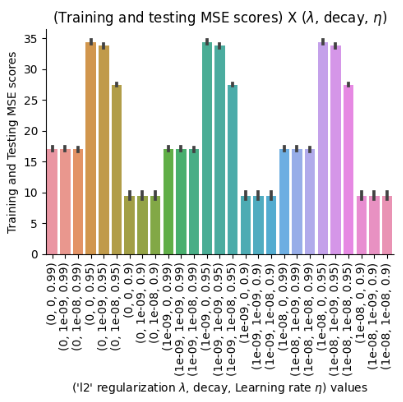
\includegraphics[height=8cm]{B11}
\caption{Bar-plot containing selected best scores for the $\eta$, decay and $\lambda$ parameter search. The upper extreme of the black bars is the testing MSE scores, and the lower extreme of the same black bars is the training MSE scores. The colored bars are the average between training and testing MSE scores.}
\end{figure}

The \hyperref[fig:B8]{bar-plotting above} shows that the 'l2' regularization and decay did not produce any furtherance in the best score. Although, parameters ($\lambda$=1e-9, decay=1e-9, $\eta$=0.9) and ($\lambda$=1e-8, decay=1e-8, $\eta$=0.9) achieved pretty close scores to ($\lambda$=0, decay=0, $\eta$=0.9). Since $\lambda$ attenuates the variance and avoids over-estimations and over-fitting of the model, those sets of parameters with $\lambda$ different from 0 might be better choice.

\begin{figure}[H]
\label{fig:B9}
\centering
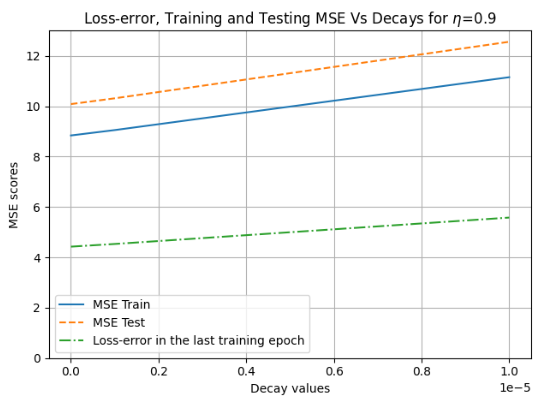
\includegraphics[height=5.5cm]{B12}
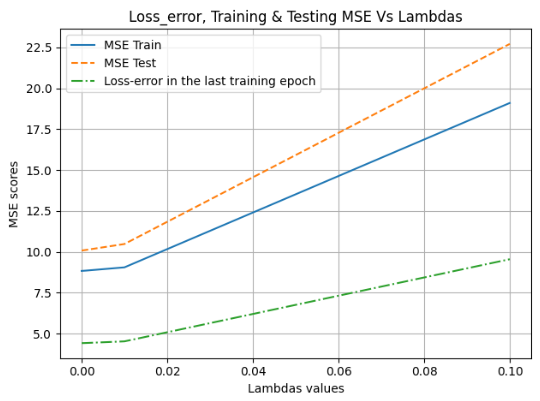
\includegraphics[height=5.5cm]{B13}
\caption{Line-plots containing loss-error, training and testing MSE as a function of decays (left), loss-error, training and testing MSE as a function of lambdas (right).}
\end{figure}

The \hyperref[fig:B9]{line-plots above} confirm that the MSE scores did not improve by applying decay and lambda parameters.

\subsubsection{Terrain image data on 2 hidden-layers MLP-DNN}
\label{chap:Terrain image data on 2 hidden-layers MLP-DNN}

\qquad \, In this sub-section, we will continue with the same data-set of GeoTIF and analyze it on an MLP with two hidden layers. The aim here is to examine if we can achieve better accuracy scores with a higher number of hidden layers.\\

The standard parameters will still be epochs=500, batch\_size = len(X\_train), learning\_rate = 'constant', decays = 0.0, lmbds = 0.0, bias0 = 0.01, init\_weights = 'normal', act\_function = 'sigmoid', output\_act\_function = 'identity', cost\_function = 'mse', random\_state = 10.\\

First, a combination of parameters between the number of neurons equal to [5, 10, 20, 50, 100, 150, 200, 300, 400, 500] per hidden-layer and learning rates equal to [0.1, 0.09, 0.08, 0.05] is performed with results as follows:

\begin{figure}[H]
\label{fig:B10}
\centering
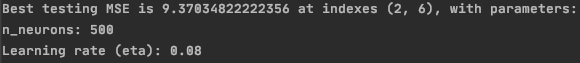
\includegraphics[width=12cm]{B14}
\caption{Output containing the best testing MSE score and its parameters.}
\end{figure}

The \hyperref[fig:B10]{output} shows that two hidden layers MLP model produces its best testing MSE score when each hidden layer has 500 neurons and eta=0.08. Catch sight on the testing MSE score obtained here (9.37) is lower and better than the score attained for one hidden layer (10.80) with 100 neurons and eta=0.9, printed in the previous section's \hyperref[fig:B1]{output}.

\begin{figure}[H]
\label{fig:B11}
\centering
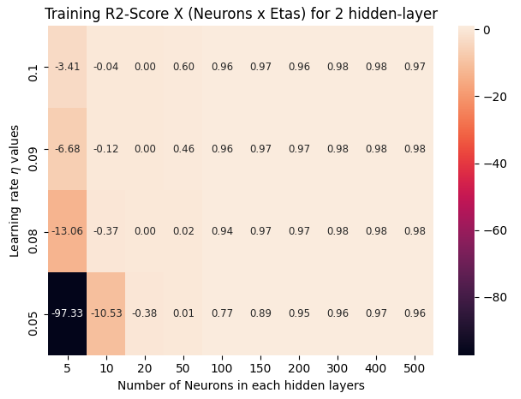
\includegraphics[height=5.5cm]{B15}
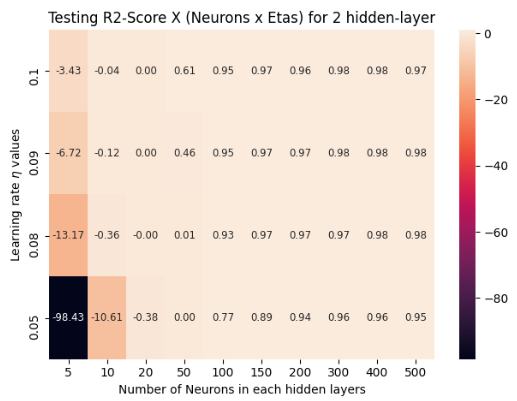
\includegraphics[height=5.5cm]{B16}
\caption{Heat-plots containing the training (left) and testing (right) R2-scores.}
\end{figure}

The R2-scores obtained for \hyperref[fig:B11]{two hidden layers} are very close to the ones attained from \hyperref[fig:B2]{one hidden layer}, but the number of neurons needs to be higher for the \hyperref[fig:B11]{former} in order to achieve the same accuracy of 0.98 from the \hyperref[fig:B2]{latter}.

\begin{figure}[H]
\label{fig:B12}
\centering
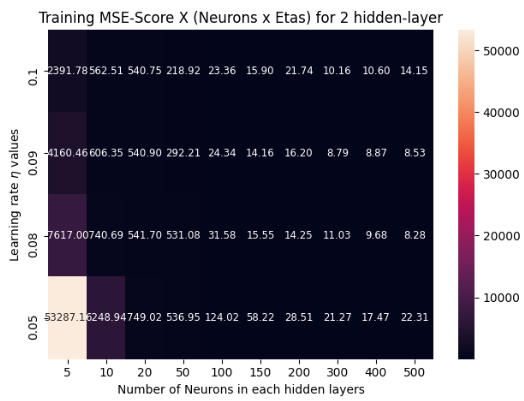
\includegraphics[height=5.5cm]{B17}
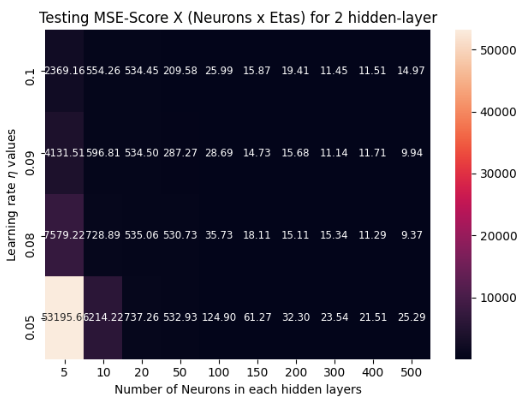
\includegraphics[height=5.5cm]{B18}
\caption{Heat-plots containing the training (left) and testing (right) MSE-scores.}
\end{figure}

The best training and testing MSE scores of 8.28 and 9.37 for \hyperref[fig:B12]{two hidden layers} are better than 8.84 and 10.09 for \hyperref[fig:B3]{one hidden layer}. This lower MSE values might owing to the fact that two hidden layers provide more significant data and complexity to the learning process, thus more accurate results. However, one must be aware that this improvement can be over-estimated or over-fitted, demanding more attention.

\begin{figure}[H]
\label{fig:B13}
\centering
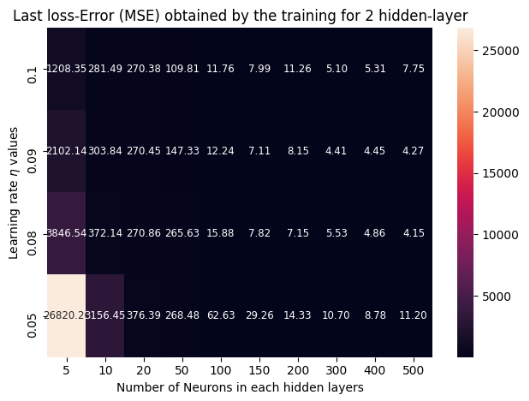
\includegraphics[height=5.5cm]{B19}
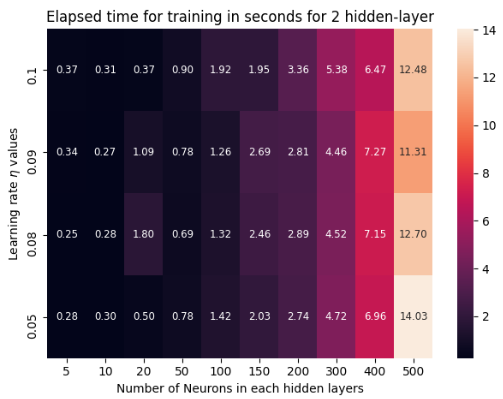
\includegraphics[height=5.5cm]{B20}
\caption{Heat-plots containing the last training loss-cost (left) and the time elapsed for training (right).}
\end{figure}

The best last training loss-error of 4.15 for \hyperref[fig:B13]{two hidden layers} are better than 4.43 for \hyperref[fig:B4]{one hidden layer}, confirming that two hidden layers perform better than one hidden layer. However, the elapsed time for training the best two hidden layers was 12.70 seconds, much higher than 0.54 seconds needed for one hidden layer.

\begin{figure}[H]
\label{fig:B14}
\centering
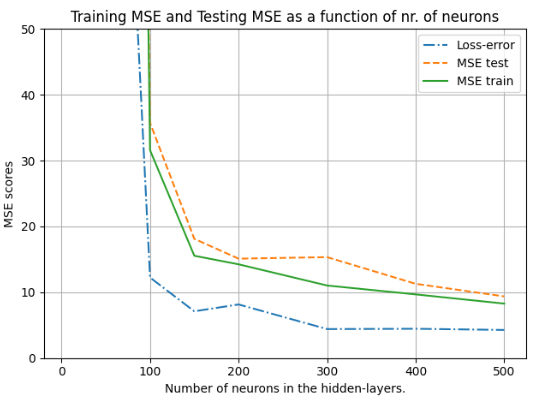
\includegraphics[height=5.5cm]{B21}
\caption{Line-plots containing the last training loss-cost, training and testing MSE scores for 100 neurons in each hidden layers and eta=0.08.}
\end{figure}

The main difference observed in the line-plots between \hyperref[fig:B14]{two hidden layers}, and \hyperref[fig:B5]{one hidden layer} is that the variance has not impacted the former, and the accuracy metric is still going under by 500 neurons. The latter has reached the lower metric score at 100 neurons, and after that, the values started to increase, showing the variance has come.

\begin{figure}[H]
\label{fig:B15}
\centering
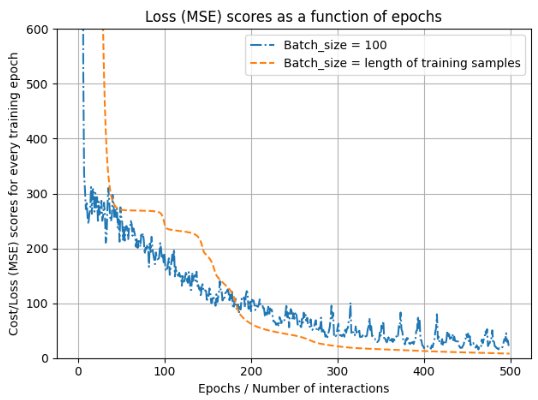
\includegraphics[height=5.5cm]{B22}
\caption{Line-plots containing the cost/loss for every epoch.}
\end{figure}

In our case, one can observe that the mini-batch strategy batch\_size=100, for \hyperref[fig:B15]{two hidden layers}, produces fewer chop bounces than for \hyperref[fig:B6]{one hidden layer}. However, the \hyperref[fig:B15]{former} takes a long time to converge to its minimum, around 300-400 epochs, while the \hyperref[fig:B6]{latter} takes 100-200 epochs.\\

\begin{figure}[H]
\label{fig:B16}
\centering
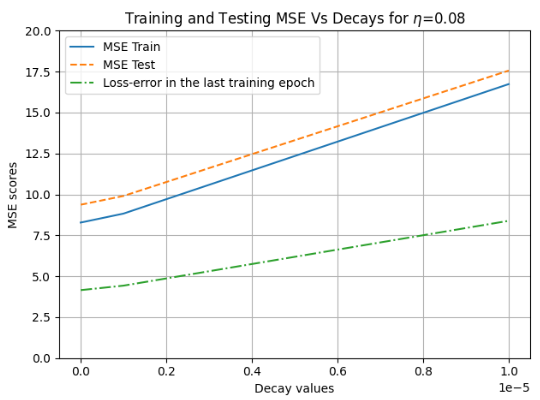
\includegraphics[height=5.5cm]{B23}
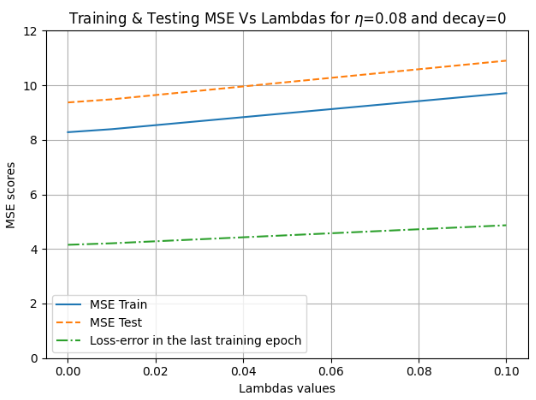
\includegraphics[height=5.5cm]{B24}
\caption{Line-plots containing learning rate = 0.08 as a function of decays = [0, 10 ** -9, 10 ** -8, 10 ** -7, 10 ** -6, 10 ** -5] (left) and lambdas = [0, 10 ** -5, 10 ** -4, 10 ** -3, 10 ** -2, 10 ** -1] (right).}
\end{figure}

Again, as happened with our \hyperref[fig:B9]{one hidden layer} MLP model, the parameters decay and lambda does not improve the model's accuracy score.\\

Finally, we perform a combination of parameters etas = [0.1, 0.09, 0.08, 0.05], decays = [0, 10 ** -9, 10 ** -8, 10 ** -7, 10 ** -6, 10 ** -5] and lambdas = [0, 10 ** -5, 10 ** -4, 10 ** -3, 10 ** -2, 10 ** -1].

\begin{figure}[H]
\label{fig:B17}
\centering
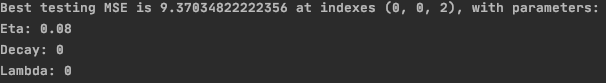
\includegraphics[width=12cm]{B25}
\caption{Output containing the result of a combination of parameters $\eta$, decay and $\lambda$.}
\end{figure}

The \hyperref[fig:B17]{output above} confirms that the parameters decay and lambda does not improve our two hidden layer MLP model's accuracy.

\subsubsection{Tanh activation function}
\label{chap:Tanh activation function}

\qquad \, Successively, we will perform the same two layer experiments done before on GeoTIF data, but now with the hyperbolic Tanh activation function for hidden layers.\\

The standard parameters will still be epochs=500, batch\_size = len(X\_train), learning\_rate = 'constant', decays = 0.0, lmbds = 0.0, bias0 = 0.01, init\_weights = 'normal', act\_function = 'tanh', output\_act\_function = 'identity', cost\_function = 'mse', random\_state = 10.\\

A combination of parameters between the number of neurons equal to [5, 10, 25, 50, 100, 150, 200, 300, 400, 500] per hidden-layer and learning rates equal to [0.3, 0.1, 0.07, 0.05, 0.04, 0.03, 0.02, 0.01] is performed with results as follows:

\begin{figure}[H]
\label{fig:B18}
\centering
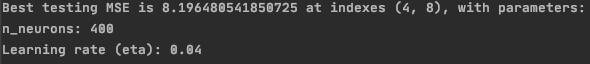
\includegraphics[width=12cm]{B26}
\caption{Output with the best testing MSE and parameters neurons and etas.}
\end{figure}

The output shows that the hyperbolic tanh for two hidden layers got its best testing MSE score of \hyperref[fig:B18]{8.19}, which is better than the best testing score for \hyperref[fig:B1]{one hidden layers Sigmoid} (10.08) or \hyperref[fig:B10]{two hidden layer Sigmoid} (9.37) experiments. This might have happened because hyperbolic tanh helps the gradient descent to not vanish, as explained in the theory section of \hyperref[chap:The vanishing or exploding gradient problems]{"the vanishing or exploding gradient problems"}.

\begin{figure}[H]
\label{fig:B19}
\centering
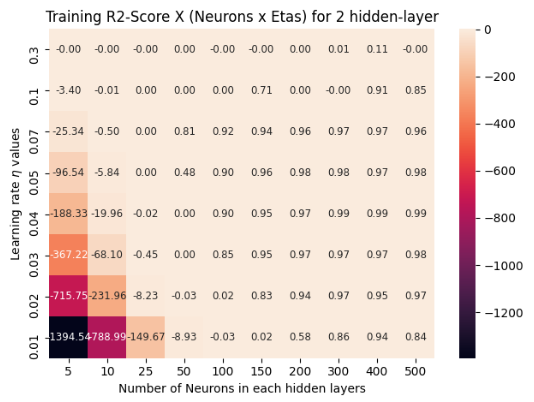
\includegraphics[height=5.5cm]{B27}
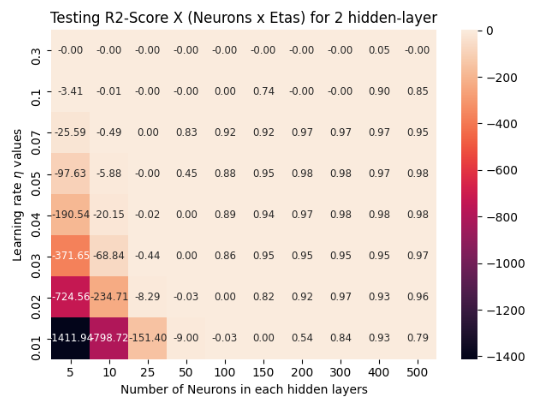
\includegraphics[height=5.5cm]{B28}
\caption{Heat-maps containing the training (left) and testing (right) R2-Scores.}
\end{figure}

The R2-scores continues very high at \hyperref[fig:B19]{0.98}, as obtained for \hyperref[fig:B11]{two hidden layers Sigmoid} or \hyperref[fig:B2]{one hidden layer Sigmoid}, showing that the MLP model is able to identify the linearity of the training data with a very good precision.

\begin{figure}[H]
\label{fig:B20}
\centering
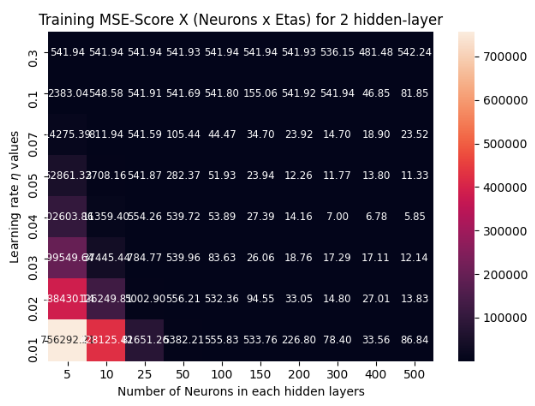
\includegraphics[height=5.5cm]{B29}
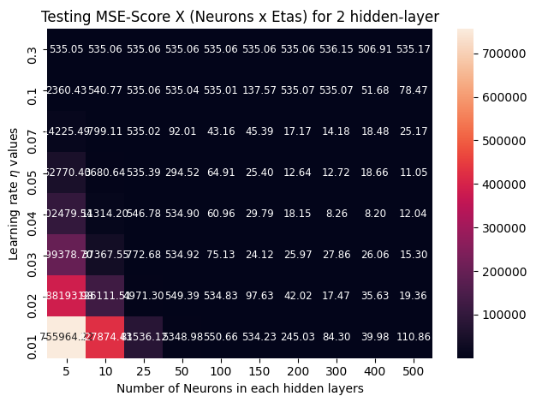
\includegraphics[height=5.5cm]{B30}
\caption{Heat-maps containing the training (left) and testing (right) MSE-Scores.}
\end{figure}

The best training and testing MSE scores of \hyperref[fig:B20]{6,78 and 8,19} are better than the ones achieved on \hyperref[fig:B12]{two hidden layers Sigmoid} (8.28 and 9.37) or \hyperref[fig:B3]{one hidden layer Sigmoid} (8.84 and 10.08), confirming that the Tanh activation function performed better than Sigmoid.

\begin{figure}[H]
\label{fig:B21}
\centering
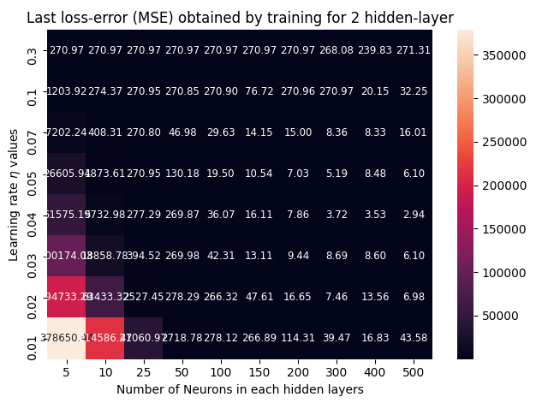
\includegraphics[height=5.5cm]{B31}
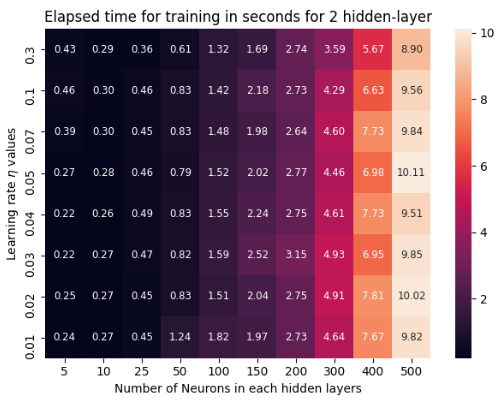
\includegraphics[height=5.5cm]{B32}
\caption{Heat-maps containing the loss-error at last epoch (left) and training elapsed times (right).}
\end{figure}

Also, observe that the loss-error for the last epoch during training with Tanh got \hyperref[fig:B21]{(2,94)} smaller scores than for \hyperref[fig:B13]{two hidden layers Sigmoid (4.15)} or for \hyperref[fig:B4]{one hidden layer Sigmoid (4.43)}.\\

Moreover, the elapsed time for training the best \hyperref[fig:B21]{two hidden layers Tanh} was 7.73 seconds, faster than 12.70 seconds for \hyperref[fig:B13]{two hidden layers Sigmoid}, but slower than 0.54 seconds for \hyperref[fig:B4]{one hidden layer Sigmoid}.

\begin{figure}[H]
\label{fig:B22}
\centering
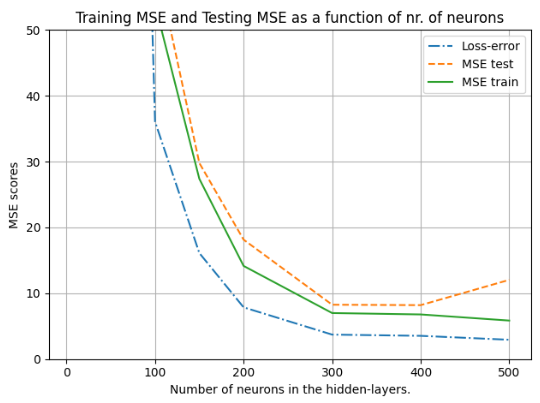
\includegraphics[height=5.5cm]{B33}
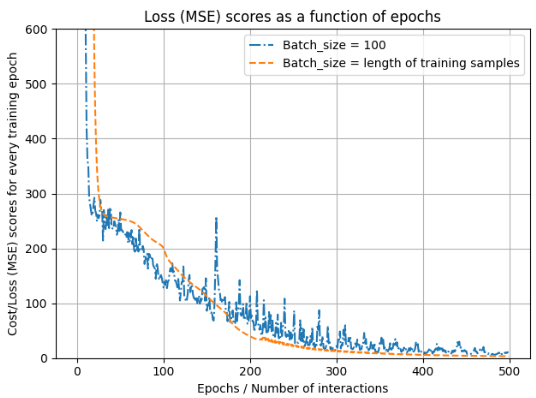
\includegraphics[height=5.5cm]{B34}
\caption{Left line-plots containing the last training loss-cost, training and testing MSE scores for 400 neurons in each hidden layers and eta=0.04. Right line-plots containing the cost/loss for every epoch.}
\end{figure}

\hyperref[fig:B22]{Left line-plots above} shows that the model reaches its minimum accuracy around 300 or 400 epochs, where we can notice an increase of the variance. Thus, be variance has come later than for \hyperref[fig:B5]{one hidden layer Sigmoid} (converged at, but earlier than for  \hyperref[fig:B14]{two hidden layers Sigmoid}.\\

Regarding the \hyperref[fig:B22]{right line-plots above}, both batch and mini-batch strategies reached its minimum around 300-400 epochs with their typical behavior, a smooth decreasing line for the first and a bounced line for the second.\\

Now, a parameter combination between learning rate = [0.1, 0.07, 0.06, 0.05, 0.04, 0.03], decays = [0, 10 ** -9, 10 ** -8, 10 ** -7, 10 ** -6, 10 ** -5] and lambdas = [0, 10 ** -5, 10 ** -4, 10 ** -3, 10 ** -2, 10 ** -1] is performed on MLP, obtaining the following results:

\begin{figure}[H]
\label{fig:B23}
\centering
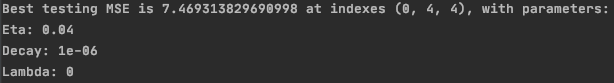
\includegraphics[width=12cm]{B35}
\caption{Output with the best testing MSE and parameters etas, decay and lambdas.}
\end{figure}

\begin{figure}[H]
\label{fig:B24}
\centering
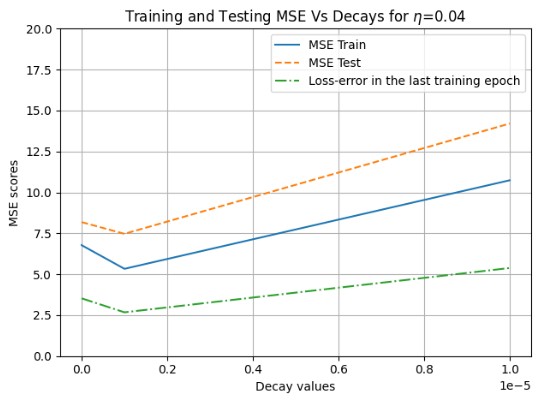
\includegraphics[height=5.5cm]{B36}
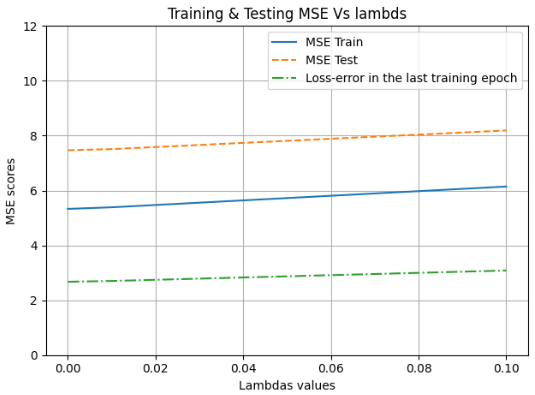
\includegraphics[height=5.5cm]{B37}
\caption{Line-plots containing learning rate = 0.04 as a function of decays = [0, 10 ** -9, 10 ** -8, 10 ** -7, 10 ** -6, 10 ** -5] (left) and lambdas = [0, 10 ** -5, 10 ** -4, 10 ** -3, 10 ** -2, 10 ** -1] (right).}
\end{figure}

One can see that the decay parameter got a positive effect resulting in an accuracy improvement on testing MSE from \hyperref[fig:B18]{8.19} to \hyperref[fig:B23]{7.46}. However, the lambda parameter has not positively impacted the results.

\subsubsection{ReLu activation function}
\label{chap:ReLu activation function}

\qquad \, In succession, we will perform the same two layer experiments done before on GeoTIF data, but now with the ReLu activation function for hidden layers.\\

The standard parameters will still be epochs=500, batch\_size = len(X\_train), learning\_rate = 'constant', decays = 0.0, lmbds = 0.0, bias0 = 0.01, init\_weights = 'normal', act\_function = 'relu', output\_act\_function = 'identity', cost\_function = 'mse', random\_state = 10.\\

A combination of parameters between the number of neurons equal to [7, 8, 9, 10, 14, 15] per hidden-layer and learning rates equal to [0.001, 0.0009, 0.0008, 0.0007, 0.0006, 0.0005, 0.0004, 0.0003, 0.0002, 0.0001] is performed with results as follows:

\begin{figure}[H]
\label{fig:B25}
\centering
\includegraphics[width=12cm]{B38}
\caption{Output with the best testing MSE and parameters neurons and etas.}
\end{figure}

The output shows that the ReLu for two hidden layers got its best testing MSE score of \hyperref[fig:B18]{14.18}, which is worse than the best testing score for \hyperref[fig:B18]{two hidden layers Tanh (8.19)} or for \hyperref[fig:B1]{one hidden layers Sigmoid (10.08)} or for \hyperref[fig:B10]{two hidden layer Sigmoid (9.37)} experiments.

\begin{figure}[H]
\label{fig:B26}
\centering
\includegraphics[height=5.5cm]{B39}
\includegraphics[height=5.5cm]{B40}
\caption{Heat-maps containing the training (left) and testing (right) R2-Scores.}
\end{figure}

The best R2-scores are slightly lower around 0.97 for two hidden layers ReLu, while \hyperref[fig:B19]{two hidden layers Tanh}, \hyperref[fig:B11]{two hidden layers Sigmoid}, and \hyperref[fig:B2]{one hidden layer Sigmoid} got 0.98.

\begin{figure}[H]
\label{fig:B27}
\centering
\includegraphics[height=5.5cm]{B41}
\includegraphics[height=5.5cm]{B42}
\caption{Heat-maps containing the training (left) and testing (right) MSE-Scores.}
\end{figure}

The best training and testing MSE scores of \hyperref[fig:B20]{21.87 and 15.57} are worse than the ones achieved on \hyperref[fig:B20]{two hidden layers Tanh (6,78 and 8,26)}, \hyperref[fig:B12]{two hidden layers Sigmoid (8.28 and 9.37)}, and \hyperref[fig:B3]{one hidden layer Sigmoid (8.84 and 10.09)}.

\begin{figure}[H]
\label{fig:B28}
\centering
\includegraphics[height=5.5cm]{B43}
\includegraphics[height=5.5cm]{B44}
\caption{Heat-maps containing the loss-error at last epoch (left) and training elapsed times (right).}
\end{figure}

The loss-error for the last epoch during training with ReLu got 10.94, which is higher/worse than \hyperref[fig:B21]{2,94 for two hidden layers Tanh}, \hyperref[fig:B13]{4.15 for two hidden layers Sigmoid} and \hyperref[fig:B4]{4.43 for one hidden layer Sigmoid}.\\

On the other hand, the elapsed time for training the best scores on ReLu is way faster at 0.30 seconds, comparing to 7.73 seconds for \hyperref[fig:B21]{two hidden layers Tanh}, 12.70 seconds for \hyperref[fig:B13]{two hidden layers Sigmoid}, and 0.54 seconds for \hyperref[fig:B4]{one hidden layer Sigmoid}.

\begin{figure}[H]
\label{fig:B29}
\centering
\includegraphics[height=5.5cm]{B45}
\includegraphics[height=5.5cm]{B46}
\caption{Left line-plots containing the last training loss-cost, training and testing MSE scores for 9 neurons in each hidden layers and eta=0.0005. Right line-plots containing the cost/loss for every epoch.}
\end{figure}

\hyperref[fig:B29]{Left line-plots above} shows that the model reaches its minimum accuracy with around 9 neurons per hidden layer, where we can notice an increase of the variance after that.\\

\hyperref[fig:B29]{Right line-plots above} exhibits that the model reaches its minimum training accuracy around 200 or 300 epochs, which is faster than \hyperref[fig:B22]{two hidden layers Tanh}, both batch and mini-batch strategies, which reached its minimum around 300-400 epochs. Still, a smooth decreasing line for the batch step and a bounced line for mini-batch step were verified.\\

Finally, a parameter combination between learning rate = [0.0006, 0.0005, 0.0004], decays = [0, 10 ** -8, 10 ** -7, 10 ** -6, 10 ** -5, 10 ** -4] and lambdas = [0, 0.01, 0.1, 0.5, 0.9, 0.95, 0.99] is performed on MLP, obtaining the following results:

\begin{figure}[H]
\label{fig:B30}
\centering
\includegraphics[width=12cm]{B47}
\caption{Output with the best testing MSE and parameters etas, decay and lambdas.}
\end{figure}

\begin{figure}[H]
\label{fig:B31}
\centering
\includegraphics[height=5.5cm]{B48}
\includegraphics[height=5.5cm]{B49}
\caption{Line-plots containing learning rate = 0.0005 as a function of decays = [0, 10 ** -8, 10 ** -7, 10 ** -6, 10 ** -5, 10 ** -4] (left) and lambdas = [0, 0.01, 0.1, 0.5, 0.9, 0.95, 0.99] (right).}
\end{figure}

One can see that the decay and lambda parameters got a positive effect resulting in an accuracy improvement on testing MSE from \hyperref[fig:B25]{14.18} to \hyperref[fig:B31]{13.50}.

\subsubsection{Initializing weights using Xavier method}
\label{chap:Initializing weights using Xavier method}

\qquad \, At the end of this part B and C, we will carry out the same two layer experiments done before on GeoTIF data, but now using the Xavier method for weights initialization and choosing Sigmoid, Tanh, and ReLu as the activation function.\\

The standard parameters will still be epochs=500, batch\_size = len(X\_train), bias0 = 0.01, init\_weights = 'xavier', output\_act\_function = 'identity', cost\_function = 'mse', random\_state = 10.\\

A combination of parameters between the number of neurons equal to [7, 9, 15, 50, 75, 100, 250, 500] per hidden-layer and learning rates equal to [0.001, 0.00075, 0.0005, 0.0004] is conducted using ReLu activation function:

\begin{figure}[H]
\label{fig:B32}
\centering
\includegraphics[width=12cm]{B50}
\caption{Output with the best testing MSE and parameters neurons and etas.}
\end{figure}

Attention to the best testing MSE score of \hyperref[fig:B32]{13.69} which is better/smaller than \hyperref[fig:B25]{14.18} obtained for normal weights initialization on MLP with ReLu.\\

Next, a parameter combination between learning rate = [0.001, 0.00075, 0.0005, 0.0004], decays = [0, 10 ** -8, 10 ** -7, 10 ** -6, 10 ** -5] and lambdas = [0, 10 ** -2, 10 ** -1, 0.5, 0.9, 0.99] is executed on MLP with ReLu and two hidden layers of 500 neurons, coming by the following results:

\begin{figure}[H]
\label{fig:B33}
\centering
\includegraphics[width=12cm]{B51}
\caption{Output with the best testing MSE and parameters etas, decay and lambdas.}
\end{figure}

The regularization of the learning rate ($\eta$) combined to the 'l2' regularization ($\lambda$) got a positive effect reducing the best testing MSE score from \hyperref[fig:B32]{13.69} to \hyperref[fig:B33]{13.68}. This reduced score is considered more reliable because its regularization techniques decrease the model's variance and over-fitting, giving less over-estimated metrics.\\

Regarding to MLP with Tanh activation function, a combination of parameters between the number of neurons equal to [5, 10, 25, 50, 100, 150, 200, 300, 400, 500] per hidden-layer and learning rates equal to [0.3, 0.1, 0.07, 0.05, 0.04, 0.03, 0.02, 0.01] is run:

\begin{figure}[H]
\label{fig:B32}
\centering
\includegraphics[width=12cm]{B52}
\caption{Output with the best testing MSE and parameters neurons and etas.}
\end{figure}

Observe that the best testing MSE score of \hyperref[fig:B32]{28.87} is higher/worse than \hyperref[fig:B18]{8.19} acquired for Gaussian weights initialization on MLP with Tanh. Xavier's initialization choice might not be a good idea in this case, except for a possible better parameter values than the ones we have examined here.\\

Then, a parameter combination between learning rate = [0.3, 0.1, 0.07, 0.05, 0.04, 0.03, 0.02, 0.01], decays = [0, 10 ** -9, 10 ** -8, 10 ** -7, 10 ** -6, 10 ** -5] and lambdas = [0, 10 ** -5, 10 ** -4, 10 ** -3, 10 ** -2, 10 ** -1] is driven on MLP with Tanh and two hidden layers with 500 neurons, getting the subsequent outcome:

\begin{figure}[H]
\label{fig:B33}
\centering
\includegraphics[width=12cm]{B53}
\caption{Output with the best testing MSE and parameters etas, decay and lambdas.}
\end{figure}

The decay parameter improved the best testing score from \hyperref[fig:B32]{28.87} to \hyperref[fig:B33]{25.51}, however it is still far worse than \hyperref[fig:B23]{7.46} got for Gaussian weights initialization.\\

Finally, a combination of parameters between the number of neurons equal to [5, 10, 20, 50, 100, 150, 200, 300, 400, 500] per hidden-layer and learning rates equal to [0.5, 0.1, 0.05, 0.01, 0.005, 0.001, 0.0005, 0.0001] is performed on MLP using Sigmoid activation function:

\begin{figure}[H]
\label{fig:B32}
\centering
\includegraphics[width=12cm]{B54}
\caption{Output with the best testing MSE and parameters neurons and etas.}
\end{figure}

The Xavier's initialization has not helped our model to increase the performance which got \hyperref[fig:B23]{228.19} as best testing MSE score, way higher/worse than \hyperref[fig:B10]{9.37} for the Gaussian initialization on two hidden layers Sigmoid. 

In addition, a parameter combination between learning rate = [0.5, 0.1, 0.05, 0.01, 0.005, 0.001, 0.0005, 0.0001], decays = [0, 10 ** -9, 10 ** -8, 10 ** -7, 10 ** -6, 10 ** -5] and lambdas = [0, 10 ** -5, 10 ** -4, 10 ** -3, 10 ** -2, 10 ** -1, 0.5] is performed on MLP and Sigmoid, obtaining the following results:

\begin{figure}[H]
\label{fig:B33}
\centering
\includegraphics[width=12cm]{B55}
\caption{Output with the best testing MSE and parameters etas, decay and lambdas.}
\end{figure}

Again, this result did not have any improvement from \hyperref[fig:B10]{9.37} for the Gaussian initialization on two hidden layers Sigmoid.

\subsection{Part D}
\label{chap:Part D}

\quad \, In our problem, we are going to work on classifying a given handwritten digit image into one of the 10 classes (0–9). So, the problem we are dealing with is essentially a Multi-class classification and to solve this we will be using the Multinomial Logistic Regression which is also known as Softmax Regression.\\

Softmax regression (or multinomial logistic regression) is a generalized version of logistic regression and is capable of handling multiple classes and instead of the sigmoid function, it uses the softmax function. The Stanford notes on Softmax regression explains this in great detail.

\subsubsection{MNIST data-set on MLP Classifier with one hidden layer and Softmax}
\label{chap:MNIST data-set on MLP Classifier with one hidden layer and Softmax}

\begin{figure}[H]
\label{fig:D0}
\centering
\includegraphics[width=12cm]{D0}
\caption{Output with the best testing accuracy for parameters neurons and etas.}
\end{figure}

\begin{figure}[H]
\label{fig:D1}
\centering
\includegraphics[height=5.5cm]{D1}
\includegraphics[height=5.5cm]{D2}
\caption{Heat-maps containing the training (left) and testing (right) Accuracy-scores.}
\end{figure}

\begin{figure}[H]
\label{fig:D2}
\centering
\includegraphics[height=5.5cm]{D3}
\includegraphics[height=5.5cm]{D4}
\caption{Heat-maps containing the training elapsed times (left), and line-plots containing the training and testing accuracies for the best parameters.}
\end{figure}

\begin{figure}[H]
\label{fig:D3}
\centering
\includegraphics[width=12cm]{D5}
\caption{Output with the best testing accuracy for parameters etas, epochs and lambdas.}
\end{figure}

\begin{figure}[H]
\label{fig:D4}
\centering
\includegraphics[height=5.5cm]{D6}
\includegraphics[height=5.5cm]{D7}
\caption{Line-plots containing learning rate = 0.1 as a function of epochs = [10, 20, 40, 60, 80, 100, 120, 140, 160, 180, 200] (left) and lambdas = [0, 10**-9, 10 ** -7, 10 ** -5, 10 ** -3, 10 ** -1, 0.5] (right).}
\end{figure}

\subsubsection{MNIST data-set on MLP Classifier with two hidden layer and Softmax}
\label{chap:MNIST data-set on MLP Classifier with two hidden layer and Softmax}

\begin{figure}[H]
\label{fig:D5}
\centering
\includegraphics[width=12cm]{D8}
\caption{Output with the best testing accuracy for parameters neurons and etas.}
\end{figure}

\begin{figure}[H]
\label{fig:D6}
\centering
\includegraphics[height=5.5cm]{D9}
\includegraphics[height=5.5cm]{D10}
\caption{Heat-maps containing the training (left) and testing (right) Accuracy-scores.}
\end{figure}

\begin{figure}[H]
\label{fig:D7}
\centering
\includegraphics[height=5.5cm]{D11}
\includegraphics[height=5.5cm]{D12}
\caption{Heat-maps containing the training elapsed times (left), and line-plots containing the training and testing accuracies for the best parameters.}
\end{figure}

\begin{figure}[H]
\label{fig:D8}
\centering
\includegraphics[width=12cm]{D13}
\caption{Output with the best testing accuracy for parameters etas, epochs and lambdas.}
\end{figure}

\begin{figure}[H]
\label{fig:D9}
\centering
\includegraphics[height=5.5cm]{D14}
\includegraphics[height=5.5cm]{D15}
\caption{Line-plots containing learning rate = 0.2 as a function of epochs = [10, 20, 40, 60, 80, 100, 120, 140, 160, 180, 200] (left) and lambdas = [0, 10**-9, 10 ** -7, 10 ** -5, 10 ** -3, 10 ** -1, 0.5] (right).}
\end{figure}

\subsubsection{MNIST data-set on MLP Classifier with one hidden layer and Sigmoid}
\label{chap:MNIST data-set on MLP Classifier with one hidden layer and Sigmoid}

\begin{figure}[H]
\label{fig:D10}
\centering
\includegraphics[width=12cm]{D16}
\caption{Output with the best testing accuracy for parameters neurons and etas.}
\end{figure}

\begin{figure}[H]
\label{fig:D11}
\centering
\includegraphics[height=5.5cm]{D17}
\includegraphics[height=5.5cm]{D18}
\caption{Heat-maps containing the training (left) and testing (right) Accuracy-scores.}
\end{figure}

\begin{figure}[H]
\label{fig:D12}
\centering
\includegraphics[height=5.5cm]{D19}
\includegraphics[height=5.5cm]{D20}
\caption{Heat-maps containing the training elapsed times (left), and line-plots containing the training and testing accuracies for the best parameters.}
\end{figure}

\begin{figure}[H]
\label{fig:D13}
\centering
\includegraphics[width=12cm]{D21}
\caption{Output with the best testing accuracy for parameters etas, epochs and lambdas.}
\end{figure}

\begin{figure}[H]
\label{fig:D14}
\centering
\includegraphics[height=5.5cm]{D22}
\includegraphics[height=5.5cm]{D23}
\caption{Line-plots containing learning rate = 0.2 as a function of epochs = [10, 20, 40, 60, 80, 100, 120, 140, 160, 180, 200] (left) and lambdas = [0, 10**-9, 10 ** -7, 10 ** -5, 10 ** -3, 10 ** -1, 0.5] (right).}
\end{figure}

\subsubsection{MNIST data-set on MLP Classifier with two hidden layer and Sigmoid}
\label{chap:MNIST data-set on MLP Classifier with two hidden layer and Sigmoid}

\begin{figure}[H]
\label{fig:D15}
\centering
\includegraphics[width=12cm]{D24}
\caption{Output with the best testing accuracy for parameters neurons and etas.}
\end{figure}

\begin{figure}[H]
\label{fig:D16}
\centering
\includegraphics[height=5.5cm]{D25}
\includegraphics[height=5.5cm]{D26}
\caption{Heat-maps containing the training (left) and testing (right) Accuracy-scores.}
\end{figure}

\begin{figure}[H]
\label{fig:D17}
\centering
\includegraphics[height=5.5cm]{D27}
\includegraphics[height=5.5cm]{D28}
\caption{Heat-maps containing the training elapsed times (left), and line-plots containing the training and testing accuracies for the best parameters.}
\end{figure}

\begin{figure}[H]
\label{fig:D18}
\centering
\includegraphics[width=12cm]{D29}
\caption{Output with the best testing accuracy for parameters etas, epochs and lambdas.}
\end{figure}

\begin{figure}[H]
\label{fig:D19}
\centering
\includegraphics[height=5.5cm]{D30}
\includegraphics[height=5.5cm]{D31}
\caption{Line-plots containing learning rate = 0.2 as a function of epochs = [10, 20, 40, 60, 80, 100, 120, 140, 160, 180, 200] (left) and lambdas = [0, 10**-9, 10 ** -7, 10 ** -5, 10 ** -3, 10 ** -1, 0.5] (right).}
\end{figure}

\subsubsection{Breast Cancer data-set on MLP Classifier with one hidden layer and Softmax}
\label{chap:Breast Cancer data-set on MLP Classifier with one hidden layer and Softmax}

\begin{figure}[H]
\label{fig:D20}
\centering
\includegraphics[width=12cm]{D32}
\caption{Output with the best testing accuracy for parameters neurons and etas.}
\end{figure}

\begin{figure}[H]
\label{fig:D21}
\centering
\includegraphics[height=5.5cm]{D33}
\includegraphics[height=5.5cm]{D34}
\caption{Heat-maps containing the training (left) and testing (right) Accuracy-scores.}
\end{figure}

\begin{figure}[H]
\label{fig:D22}
\centering
\includegraphics[height=5.5cm]{D35}
\includegraphics[height=5.5cm]{D36}
\caption{Heat-maps containing the training elapsed times (left), and line-plots containing the training and testing accuracies for the best parameters.}
\end{figure}

\begin{figure}[H]
\label{fig:D23}
\centering
\includegraphics[width=12cm]{D37}
\caption{Output with the best testing accuracy for parameters etas, epochs and lambdas.}
\end{figure}

\begin{figure}[H]
\label{fig:D24}
\centering
\includegraphics[height=5.5cm]{D38}
\includegraphics[height=5.5cm]{D39}
\caption{Line-plots containing learning rate = 0.2 as a function of epochs = [10, 20, 40, 60, 80, 100, 120, 140, 160, 180, 200] (left) and lambdas = [0, 10**-9, 10 ** -7, 10 ** -5, 10 ** -3, 10 ** -1, 0.5] (right).}
\end{figure}

\subsubsection{Breast Cancer data-set on MLP Classifier with one hidden layer and Sigmoid}
\label{chap:Breast Cancer data-set on MLP Classifier with one hidden layer and Sigmoid}

\begin{figure}[H]
\label{fig:D25}
\centering
\includegraphics[width=12cm]{D40}
\caption{Output with the best testing accuracy for parameters neurons and etas.}
\end{figure}

\begin{figure}[H]
\label{fig:D26}
\centering
\includegraphics[height=5.5cm]{D41}
\includegraphics[height=5.5cm]{D42}
\caption{Heat-maps containing the training (left) and testing (right) Accuracy-scores.}
\end{figure}

\begin{figure}[H]
\label{fig:D27}
\centering
\includegraphics[height=5.5cm]{D43}
\includegraphics[height=5.5cm]{D44}
\caption{Heat-maps containing the training elapsed times (left), and line-plots containing the training and testing accuracies for the best parameters.}
\end{figure}

\begin{figure}[H]
\label{fig:D28}
\centering
\includegraphics[width=12cm]{D45}
\caption{Output with the best testing accuracy for parameters etas, epochs and lambdas.}
\end{figure}

\begin{figure}[H]
\label{fig:D29}
\centering
\includegraphics[height=5.5cm]{D46}
\includegraphics[height=5.5cm]{D47}
\caption{Line-plots containing learning rate = 0.2 as a function of epochs = [10, 20, 40, 60, 80, 100, 120, 140, 160, 180, 200] (left) and lambdas = [0, 10**-9, 10 ** -7, 10 ** -5, 10 ** -3, 10 ** -1, 0.5] (right).}
\end{figure}

\subsection{Part E}
\label{chap:Part E}
